\chapter{Análisis de Resultados}
\section{Capturas del programa en ejecución}

A continuación se presenta en orden el proceso de ejecución del programa, donde primeramente se muestra el código en ejecución para la parte de la animación y otro ejemplo más grande donde no se incluye animación.\newline
\newpage

\begin{enumerate}
\item Iniciamos el programa, donde nos pide que introduzcamos una opción en el menú de inicio, seleccionamos opción 1 y luego digitamos '0011' que será nuestra cadena a evaluar. El programa nos indica que la cadena fue evaluada y es valida. Observar la Figura 2.1.

\begin{figure}[h]
%\begin{minipage}{0.3\textwidth}
    \begin{center}
    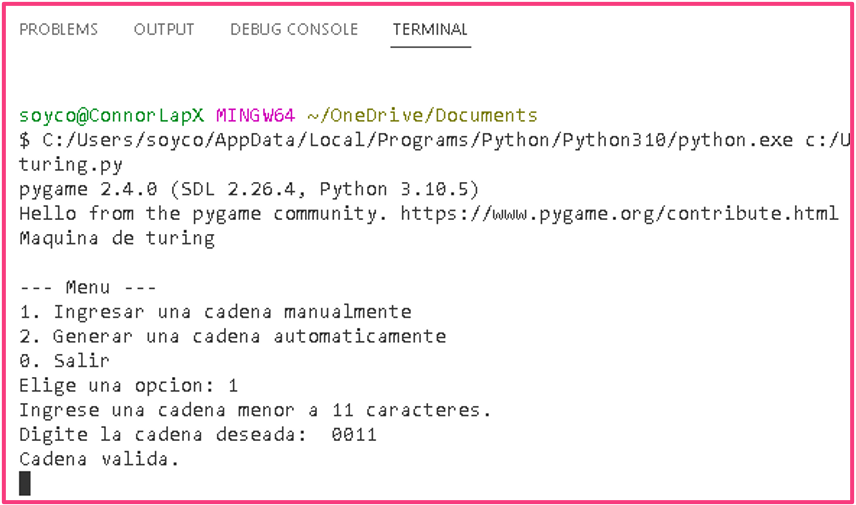
\includegraphics[width=0.8\linewidth]{Images/Cap8.png}
    \end{center}
%\end{minipage}
\caption{Visualización del programa en terminal caso 1.}
\label{fig:imagen}
\end{figure}
\newpage
\item Aquí se puede ver la primera parte de la animación, donde vemos todos las transiciones de la animación, esta animación va cambiando conforme le demos clic al botón 'siguiente'.  Observar la Figura 2.2.\newline
\begin{figure}[h]
%\begin{minipage}{0.3\textwidth}
    \begin{center}
    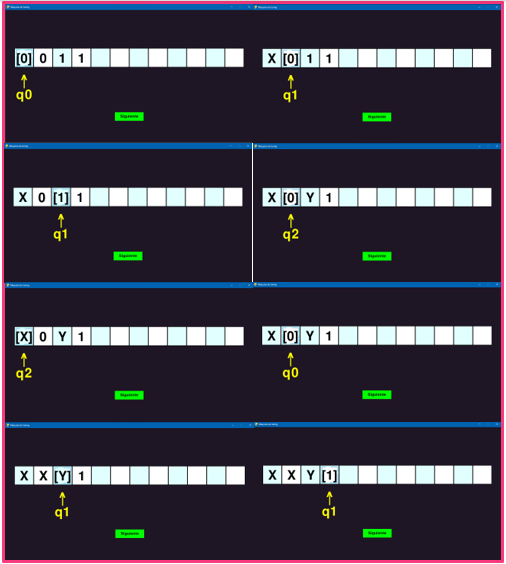
\includegraphics[width=0.8\linewidth]{Images/Cap1.png}
    \end{center}
%\end{minipage}
\caption{Visualización de la primera parte de animaciones.}
\label{fig:imagen}
\end{figure}

\newpage
\item Aquí se puede ver la segunda parte de la animación, donde vemos todos las transiciones de la animación, esta animación va cambiando conforme le demos clic al botón 'siguiente'. En esta última parte podemos ver como llegamos al estado final q4, ya si el programa finaliza. Observar la Figura 2.3.
\begin{figure}[h]
%\begin{minipage}{0.3\textwidth}
    \begin{center}
    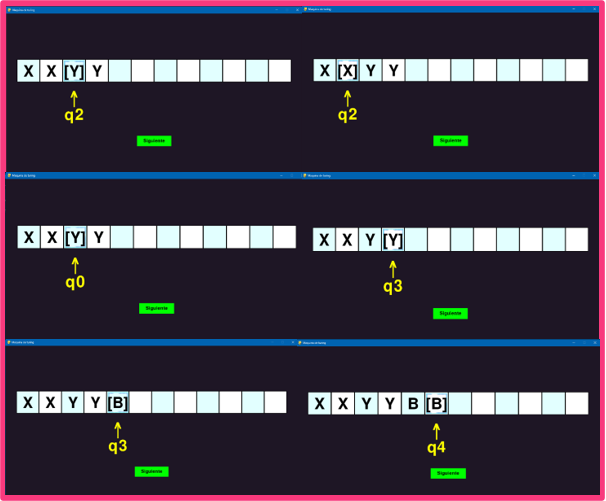
\includegraphics[width=0.8\linewidth]{Images/Cap2.png}
    \end{center}
%\end{minipage}
\caption{Visualización de la segunda parte de animaciones.}
\label{fig:imagen}
\end{figure}

\newpage
\item Aquí podemos ver el archivo de salida turing.txt, que nos mostrara cada paso de las evaluaciones de la máquina de turing. Observar la Figura 2.4.
\begin{figure}[h]
%\begin{minipage}{0.3\textwidth}
    \begin{center}
    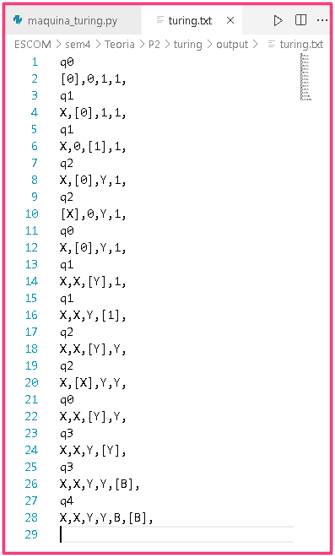
\includegraphics[width=0.5\linewidth]{Images/Cap3.png}
    \end{center}
%\end{minipage}
\caption{Vista del archivo de salida 'turing.txt'.}
\label{fig:imagen}
\end{figure}

\newpage
\item Iniciamos nuevamente el programa, esta vez seleccionamos opción 2 y nos genera una cadena aleatoria, para este caso nos genero una cadena de tamaño 446, posteriormente la evalúa y termina el programa. Observar la figura 2.5.

\begin{figure}[h]
%\begin{minipage}{0.3\textwidth}
    \begin{center}
    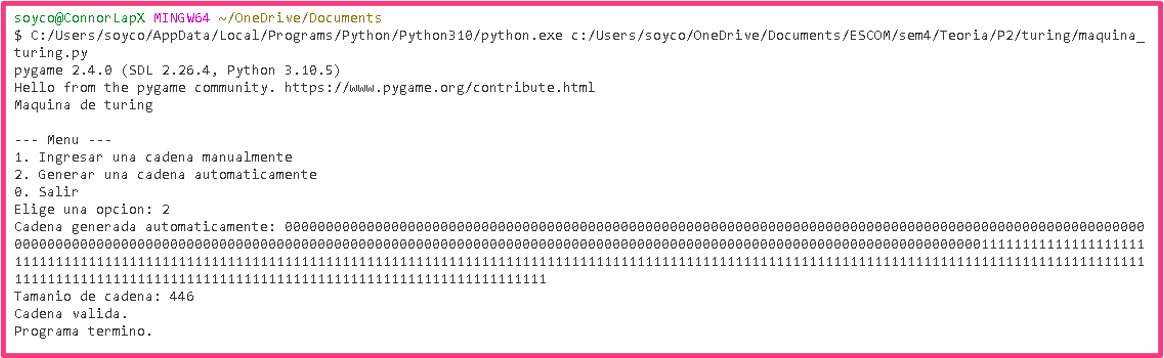
\includegraphics[width=1\linewidth]{Images/Cap4.png}
    \end{center}
%\end{minipage}
\caption{Visualización del programa en terminal caso 2.}
\label{fig:imagen}
\end{figure}

\newpage
\item Vemos que el archivo de salida 'turing.txt' llego a pesar cerca de 90MB, lo que significa que la complejidad del algoritmo incrementa exponencialmente conforme el tamaño de la cadena crece y por ende entre mayor tamaño de cadena, más recursos de memoria serán necesarios. Observar la figura 2.6.

\begin{figure}[h]
%\begin{minipage}{0.3\textwidth}
    \begin{center}
    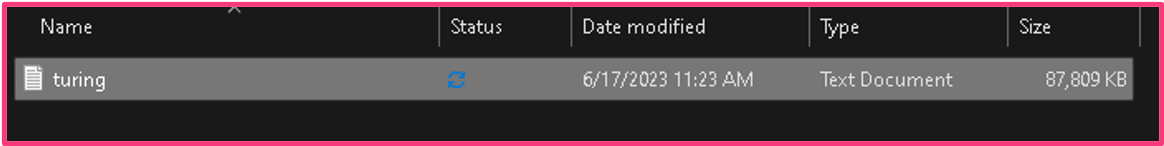
\includegraphics[width=1\linewidth]{Images/Cap5.png}
    \end{center}
%\end{minipage}
\caption{Visualización de memoria utilizada por el archivo para caso 2.}
\label{fig:imagen}
\end{figure}
\newpage
\item Aquí se puede ver el inicio del archivo de 'turing.txt', donde podemos ver que inicia correctamente con el cabezal en la primera posición. Cabe recalcar que se tuvo que hacer uso de una herramienta especial para abrir archivos grandes de información. Observar la figura 2.7.

\begin{figure}[h]
%\begin{minipage}{0.3\textwidth}
    \begin{center}
    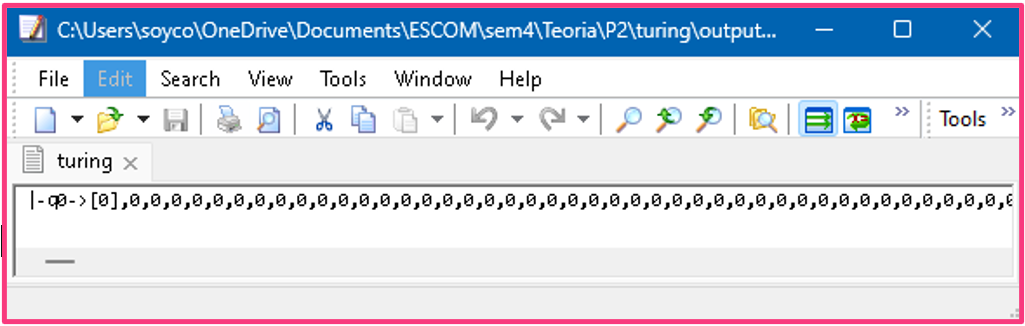
\includegraphics[width=1\linewidth]{Images/Cap6.png}
    \end{center}
%\end{minipage}
\caption{Visualización del inicio de archivo de salida turing.txt.}
\label{fig:imagen}
\end{figure}
\newpage
\item Aquí se puede ver el final del archivo de 'turing.txt', donde podemos ver en la primer parte como termina correctamente con los dos espacios en blanco, que nos indica que se llegó al estado q4, y en la parte inferior podemos ver como realmente todos los ceros y unos fueron reescritos correctamente. Observar la figura 2.7.

\begin{figure}[h]
%\begin{minipage}{0.3\textwidth}
    \begin{center}
    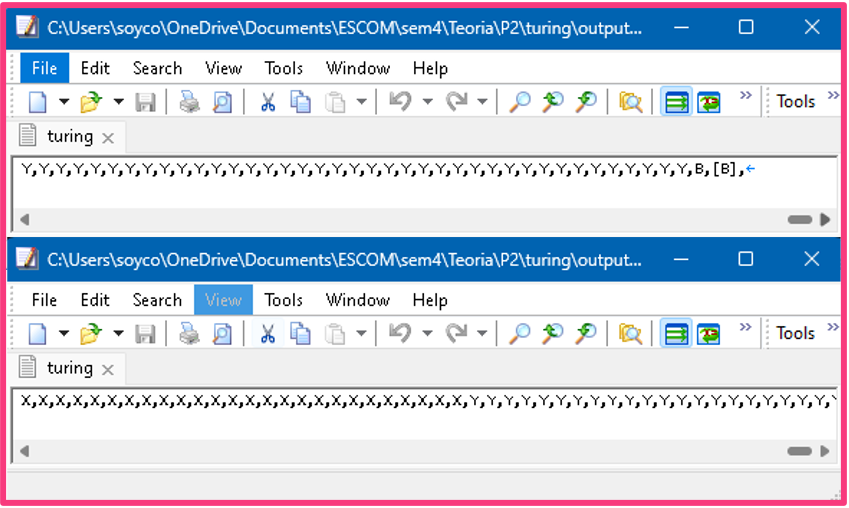
\includegraphics[width=1\linewidth]{Images/Cap7.png}
    \end{center}
%\end{minipage}
\caption{Visualización del final de archivo de salida turing.txt.}
\label{fig:imagen}
\end{figure}
\end{enumerate}